\section{Description des mises en situation}

Dans cette section, nous détaillons la mise en pratique des différents outils de gestion de projet. Pour chaque point, nous fournissons une explication de notre démarche ainsi que les captures d'écran justificatives.

\subsection*{[A1] Constitution d'un groupe \& [A3] Intégration des contributions}
Notre groupe est constitué de deux étudiants[cite: 11]. Afin de garantir une répartition équilibrée du travail[cite: 22], nous avons alterné les développements et les validations. L'historique des commits sur la branche principale montre clairement l'intégration régulière des contributions de chacun[cite: 21].

\begin{figure}[h]
    \centering
    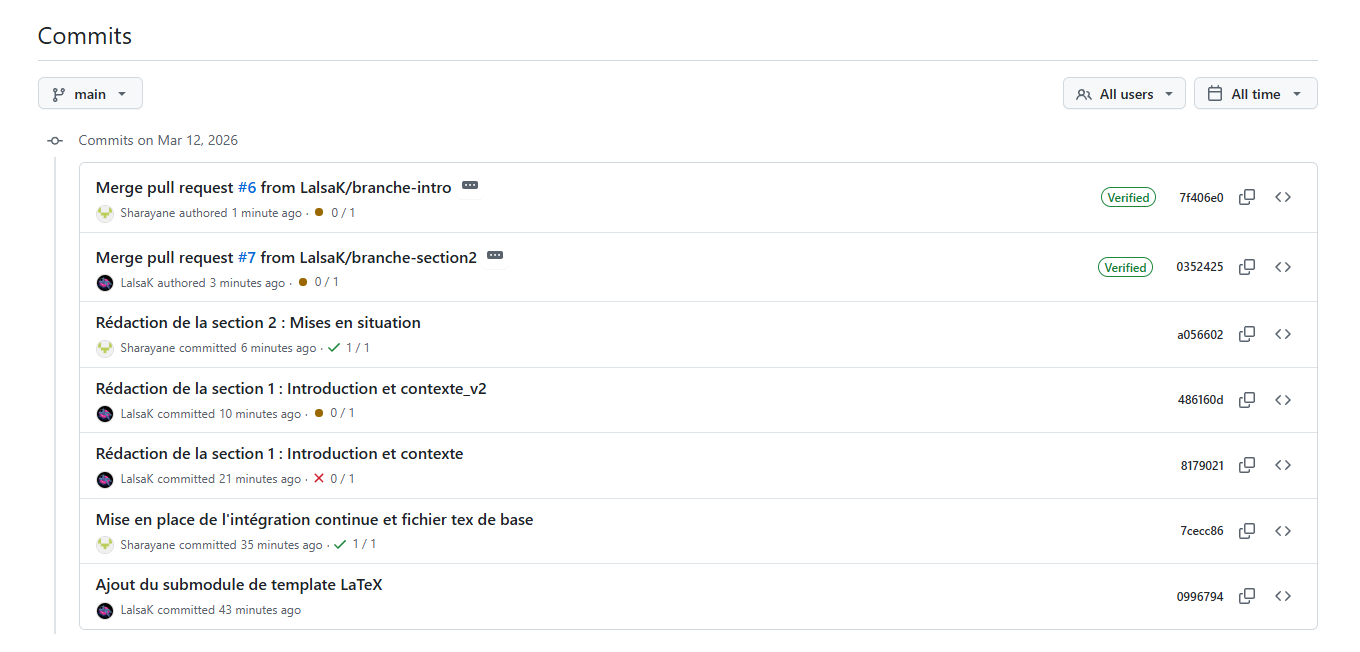
\includegraphics[width=0.8\textwidth]{images\7-Historique_commits.png}
    \caption{Historique des commits illustrant nos contributions respectives.}
\end{figure}

\subsection*{[A2] Dépôt Git en ligne}
Nous avons créé un dépôt en ligne nommé \textbf{gestion-projet-lyon2} sur la plateforme GitHub[cite: 19]. Ce dépôt étant privé pour la durée du développement, nous avons explicitement ajouté notre enseignant de CM en tant que collaborateur afin qu'il puisse y accéder et vérifier notre travail[cite: 20].


    \centering
    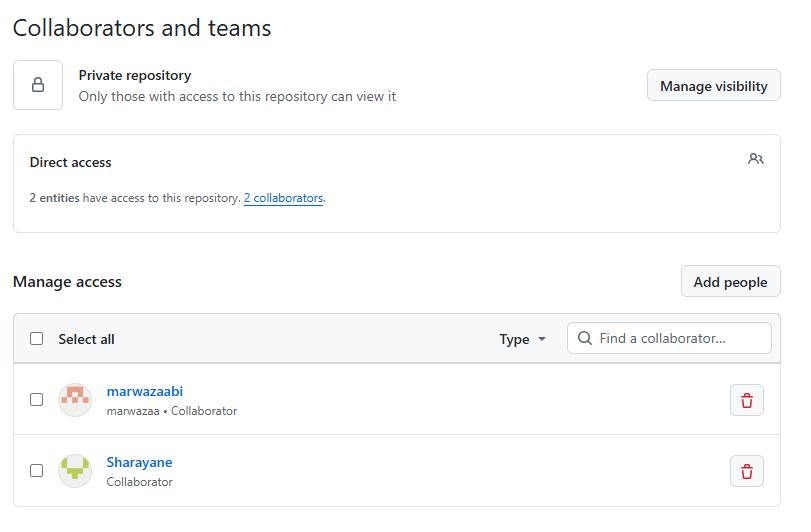
\includegraphics[width=0.8\textwidth]{images\Collaborateurs.png}
    \caption{Accès accordé à l'enseignant dans les paramètres du dépôt.}
\end{figure}

\subsection*{[B1] Gestion par branches \& [B3] Propositions de contributions}
Pour éviter les conflits lors de la rédaction de ce compte rendu, nous avons utilisé des branches séparées pour nos axes de développement [cite: 23] (ex: \texttt{feature-intro} et \texttt{feature-section2}). Chaque fusion vers la branche principale a fait l'objet d'une \textit{Pull Request} (PR) sur GitHub[cite: 27]. Cela nous a permis d'effectuer des relectures croisées et d'interagir via les commentaires avant de valider le travail de l'autre[cite: 28].

\begin{figure}[h]
    \centering
    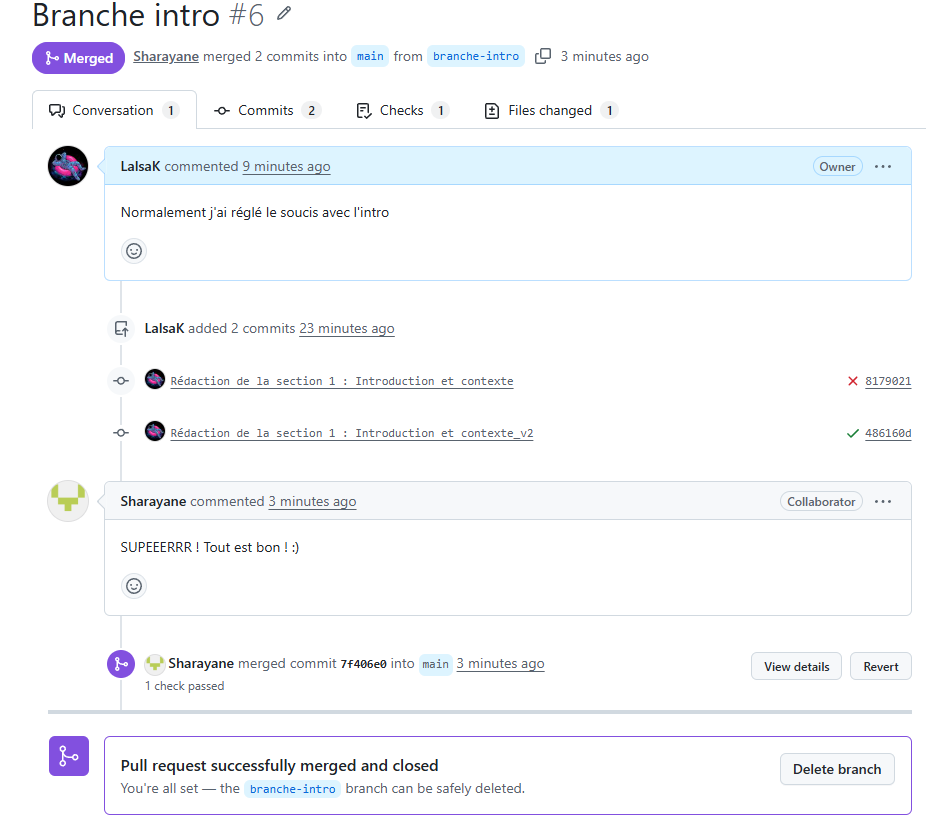
\includegraphics[width=0.8\textwidth]{images\8.1-PR_Intro.png}
    \caption{Pull Request de l'introduction.}
\end{figure}

\begin{figure}[h]
    \centering
    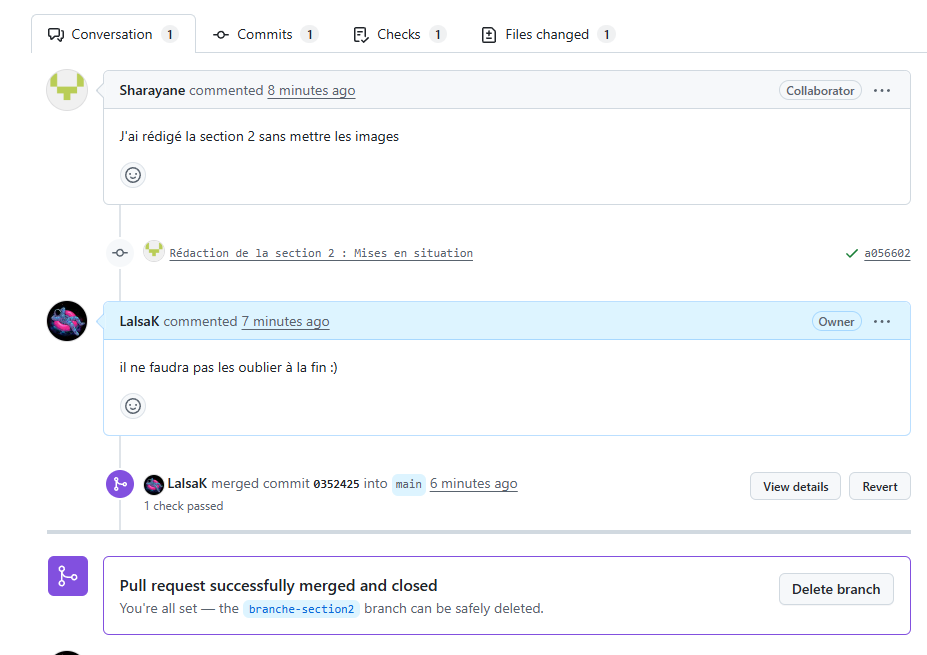
\includegraphics[width=0.8\textwidth]{images\8.2-PR_Section2.png}
    \caption{Pull Request de la section2.}
\end{figure}

\subsection*{[C1] Répartition de tâches et milestone \& [C4] Outil Projet (Kanban)}
La coordination de notre projet a été structurée autour de l'outil \textit{GitHub Projects}[cite: 40]. Nous avons créé un tableau Kanban permettant de suivre l'avancement[cite: 40]. L'ensemble de nos tâches a été défini via des \textit{Issues}, assignées à l'un ou l'autre des membres, et associées à un \textit{Milestone} spécifique pour notre rendu final[cite: 32].

\begin{figure}[h]
    \centering
    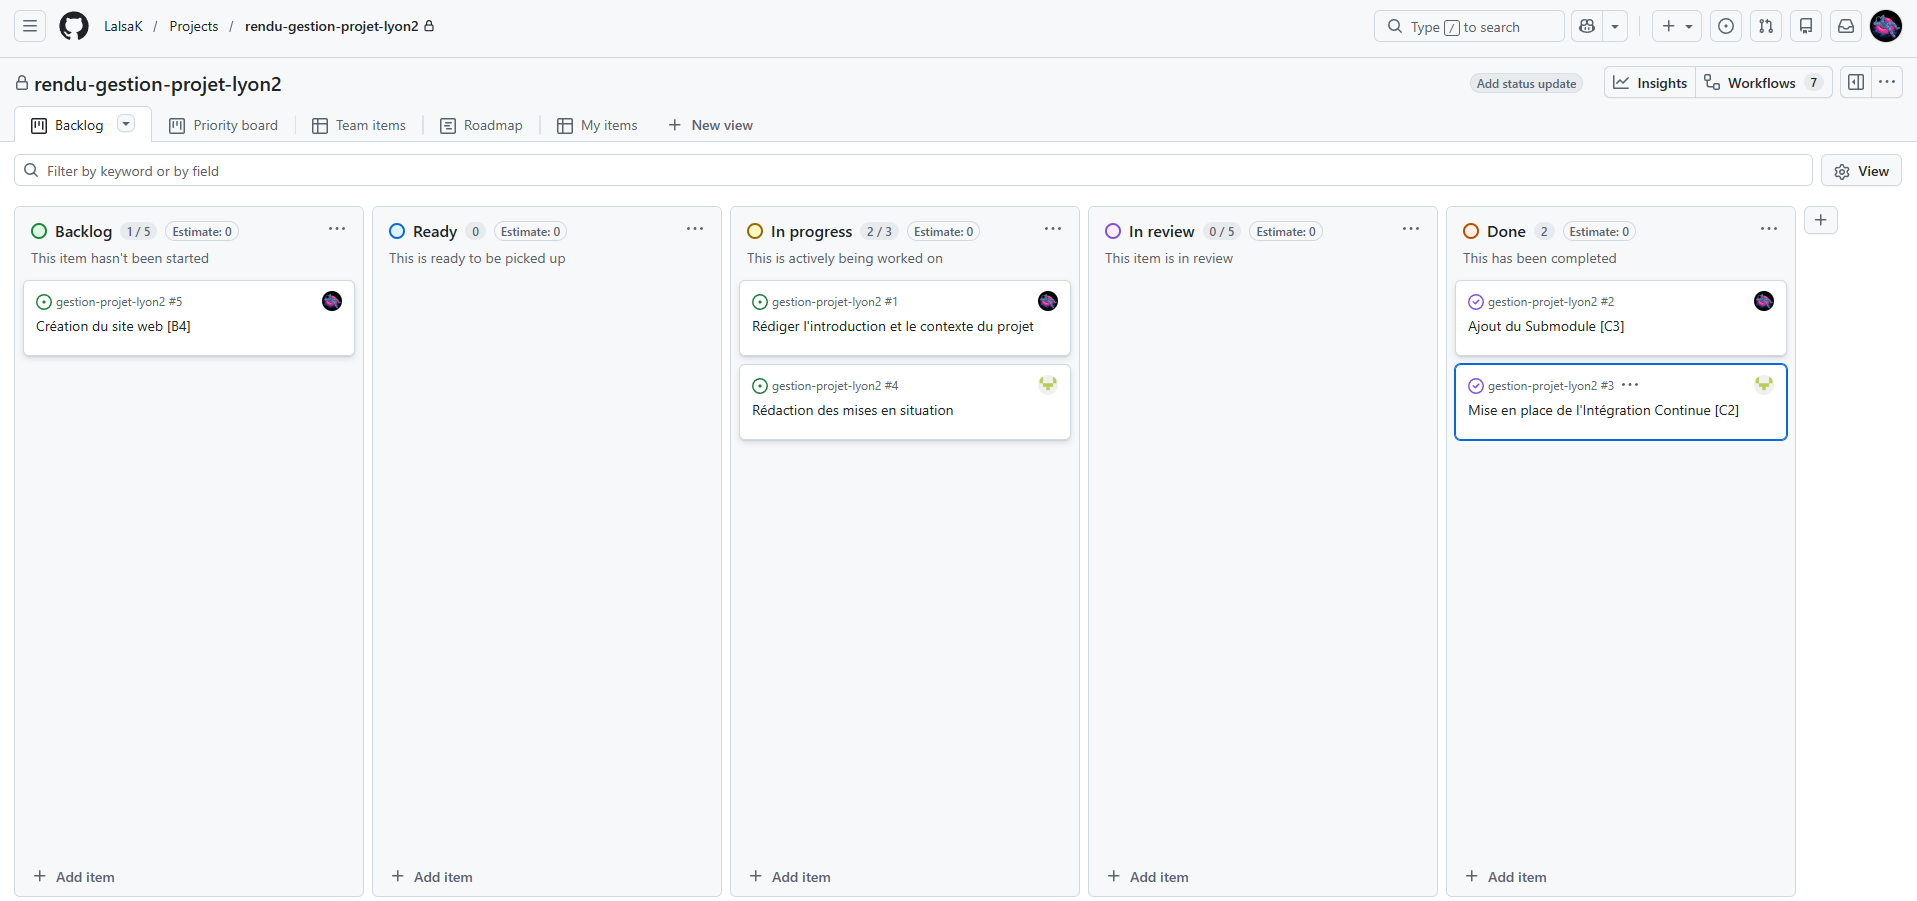
\includegraphics[width=0.8\textwidth]{images\9-Kanban_a_Jour.png}
    \caption{Tableau Kanban et répartition des tâches via les Issues.}
\end{figure}

\subsection*{[C2] Intégration continue}
Nous avons mis en place un processus d'intégration continue via \textit{GitHub Actions}[cite: 34]. À chaque nouveau \textit{push} sur la branche principale, un script se déclenche automatiquement pour compiler notre code source \LaTeX{} et générer le document PDF final[cite: 35].

\begin{figure}[h]
    \centering
    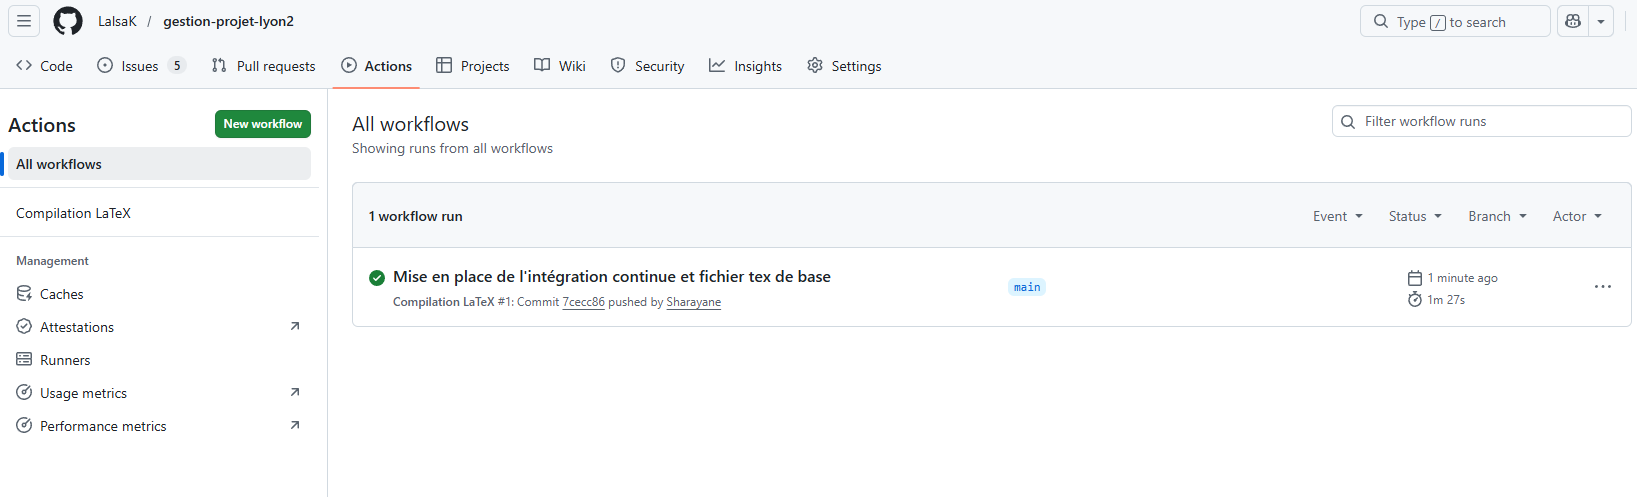
\includegraphics[width=0.8\textwidth]{images\6-Intégration_continue.png}
    \caption{Exécution réussie de l'intégration continue pour la compilation \LaTeX.}
\end{figure}

\subsection*{[C3] Gestion de submodule}
Pour démontrer notre capacité à gérer une dépendance externe[cite: 36], nous avons intégré un \textit{submodule} Git à notre projet. Il s'agit d'un répertoire de templates \LaTeX{} \textit{open source}[cite: 39]. L'enseignant peut récupérer l'intégralité du projet, incluant cette dépendance, en utilisant la commande \texttt{git clone --recursive}[cite: 37].

\begin{figure}[h]
    \centering
    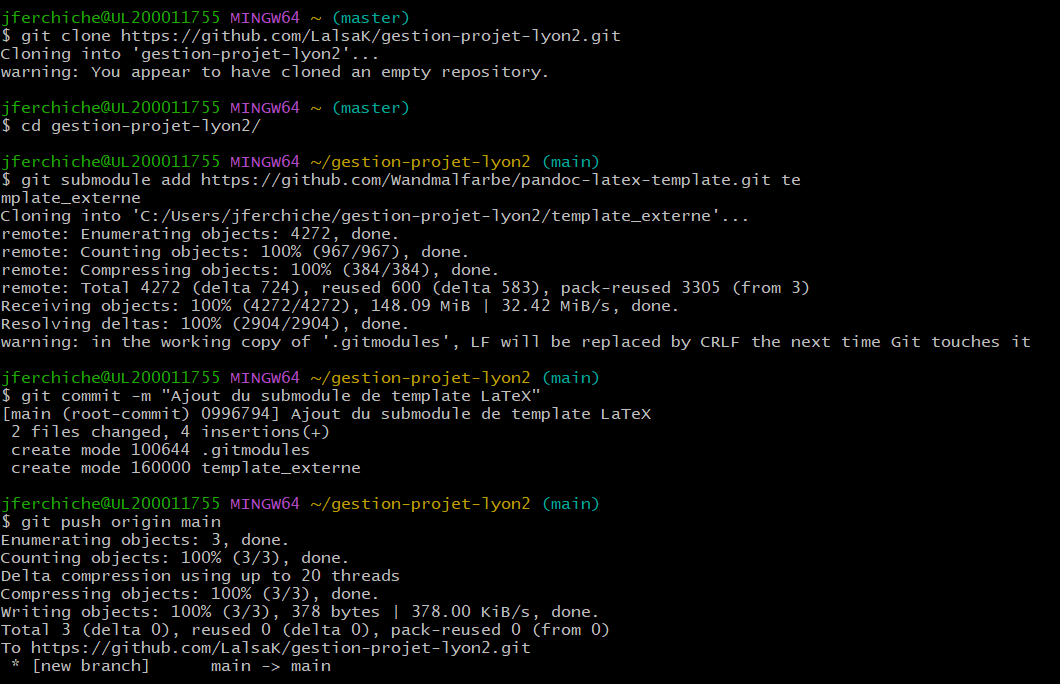
\includegraphics[width=0.8\textwidth]{images\5-Submodules.png}
    \caption{Ajout de la dépendance externe via un submodule Git.}
\end{figure}

\subsection*{[B2] Intégration de version et tag \& [B4] Intégration de site web}
Enfin, pour finaliser notre projet, nous avons déployé une page web de présentation via \textit{GitHub Pages}.
L'URL de notre site est la suivante : \url{https://github.com/LalsaK/gestion-projet-lyon2.git}
De plus, la version finale de ce document a été figée dans l'historique à l'aide d'un tag Git (version \texttt{v1.0}).

\begin{figure}[h]
\centering
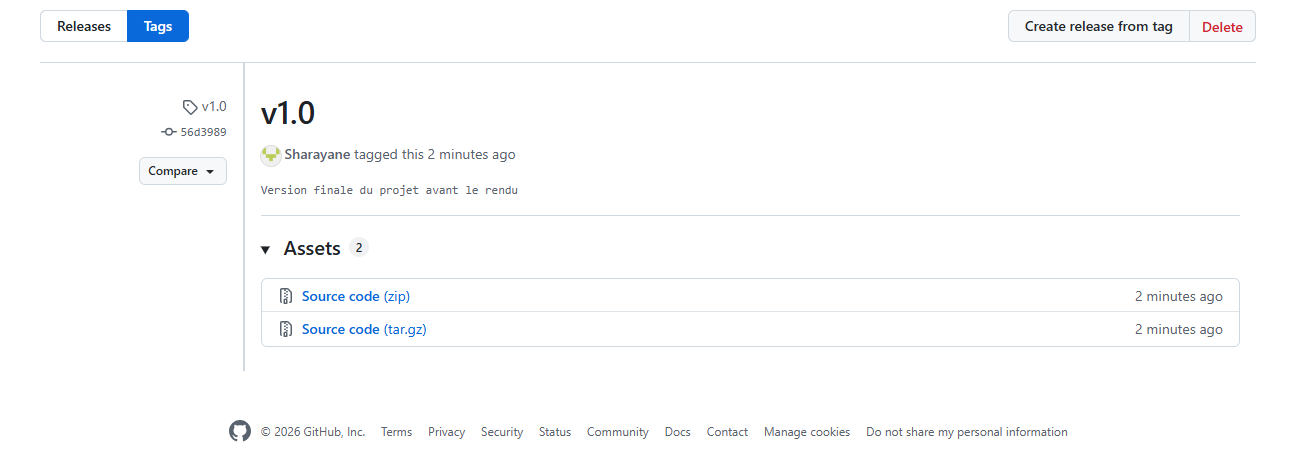
\includegraphics[width=0.45\textwidth]{images\11-Tag.png}
\hfill

\includegraphics[width=0.45\textwidth]{images\10-SiteWeb.png}
\caption{Création du tag de version finale (gauche) et déploiement du site web (droite).}
\end{figure}

